\section{需求流程与数据分析}
\label{sec:data}

\subsection{需求场景及诈骗行为特征分析}

正常交易通常具有稳定的设备、IP、时间、金额和收款习惯；诈骗交易则常表现为陌生设备登录、金额突然偏离、短时高频、多账户共享资源、资金集中流向高风险收款方等异常。系统据此将业务需求转换为“事件接入、实时特征提取、多证据融合、双阈值处置、证据链溯源、人工反馈迭代”六个连续步骤，并以低风险放行、中风险复核和高风险拦截作为最终业务输出。

\begin{figure}[H]
  \centering
  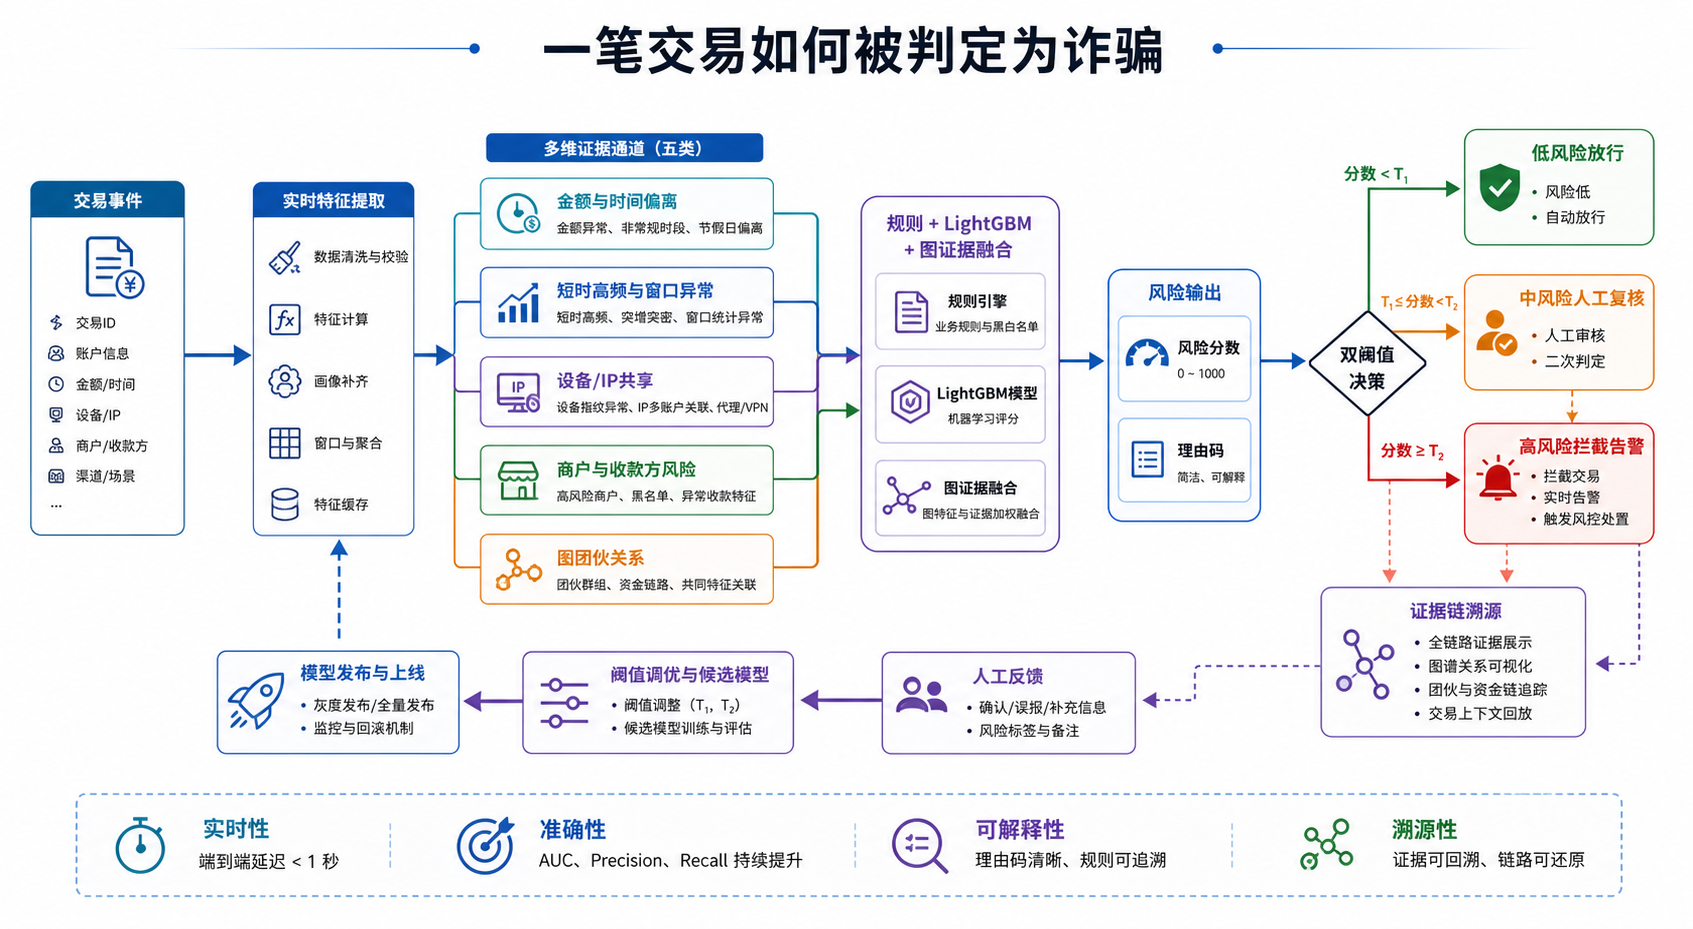
\includegraphics[width=0.98\textwidth]{pic/fraud_decision_logic_image2.png}
  \caption{一笔交易的诈骗判定、处置与反馈业务流程}
  \label{fig:fraud_decision_logic}
\end{figure}

\subsection{数据集分析}

\subsubsection{多源异构数据设计}

赛题一要求参赛团队自建或模拟包含多源异构金融交易数据的仿真环境。受金融隐私、机构安全和标签成本限制，单一公开数据集通常只能覆盖交易、身份、设备或图关系中的一部分。因此，FP-FraudSim没有简单纵向拼接原始文件，而是对八个公开或合成数据源进行``角色化融合''：交易型数据进入统一交易事实表，身份与设备字段进入特征侧表，网络型数据进入异构图，仿真器与反洗钱数据用于补充复杂欺诈模式。PaySim与BankSim提供支付仿真和消费网络\cite{paysim,banksim}，IEEE-CIS与Credit Card Fraud提供高维表格特征和类别不平衡对照\cite{ieeecis,creditcard}，Elliptic与DGraph-Fin提供资金流和金融关系图\cite{elliptic,dgraphfin}，SAML-D与AMLSim提供反洗钱交易及模式生成参考\cite{samld,amlsim}。

\begin{table}[H]
  \centering
  \caption{八个公开数据源的角色化融合方式}
  \label{tab:dataset_roles}
  \renewcommand\arraystretch{1.38}
  \setlength{\tabcolsep}{4.5pt}
  {\songti\zihao{5}
  \arrayrulecolor{tableline}
  \rowcolors{2}{tablealt}{white}
  \begin{tabularx}{0.98\textwidth}{>{\raggedright\arraybackslash}p{2.1cm}>{\raggedright\arraybackslash}p{3.1cm}>{\raggedright\arraybackslash}X>{\raggedright\arraybackslash}p{3.1cm}}
    \rowcolor{tablehead}
    \color{white}\bfseries 数据源 & \color{white}\bfseries 数据属性 & \color{white}\bfseries 在FP-FraudSim中的作用 & \color{white}\bfseries 主要产物 \\
    \specialrule{0.8pt}{0pt}{0pt}
    PaySim & 移动支付、转账、提现与余额变化 & 构成移动支付交易骨架，保留余额变化侧表 & 交易主表、PaySim特征侧表 \\
    BankSim & 消费交易、用户属性、商户类别与网络 & 补充用户/商户画像和用户--商户关系 & 交易主表、画像、图边 \\
    IEEE-CIS & 电商支付、匿名身份、卡、地址和设备字段 & 提供电商场景及高维匿名特征 & 交易主表、IEEE特征侧表 \\
    Credit Card Fraud & 极度不平衡的匿名信用卡交易 & 用于类别不平衡和异常检测对照 & 交易主表、PCA特征侧表 \\
    Elliptic Bitcoin & 带时间步和非法标签的资金流图 & 验证资金链路溯源与图模型 & 图节点、资金流图边 \\
    DGraph-Fin & 大规模金融用户动态图与17维节点特征 & 验证关系风险传播和动态图异常检测 & 图节点、关系边、节点特征侧表 \\
    SAML-D & 大规模跨境反洗钱交易与洗钱子类型 & 补充AML模式并支持流式压测 & 交易主表 \\
    IBM AMLSim & 反洗钱仿真器及样例输出 & 提供环路、扇入扇出和跑分账户模式参考 & 样例交易、转账图边 \\
    \specialrule{0.8pt}{0pt}{0pt}
  \end{tabularx}
  }
\end{table}

FP-FraudSim以\texttt{transaction\_log.parquet}为核心交易事实表，字段覆盖交易ID、来源、时间戳、金额、交易类型、渠道、支付方式、付款方、收款方、商户、设备、IP、币种、国家地区、标签和欺诈类型；围绕交易主体构建用户、商户、设备和IP画像，并以\texttt{graph\_nodes.parquet}和\texttt{graph\_edges.parquet}描述用户--交易--收款方、共享设备/IP、商户支付、资金流和用户关系。对于IEEE-CIS的匿名高维字段、Credit Card Fraud的V1--V28、PaySim余额字段和DGraph-Fin节点向量，系统通过\texttt{feature\_store\_index.parquet}记录关联键，避免核心表过宽并保留来源专属信息。

系统进一步将静态画像和动态事件分离。静态画像记录账户年龄、历史交易量、平均金额、常用设备数、常用IP数、商户投诉率、设备绑定用户数、IP代理/VPN标记等信息；动态事件记录交易时间、金额、渠道、设备、IP、商户和收款方。在线识别时，Flink从Kafka读取动态事件，再从Redis按实体ID补齐画像，使模型输入既包含单笔交易上下文，也包含历史行为基线。

\subsubsection{统一数据集构建与统计分析}

数据构建由\path{scripts/scripts/etl}下的四阶段脚本完成。首先，\path{01_normalize.py}读取CSV与NPZ文件，将不同来源映射到统一最小交易语义，并将高维或源专属字段写入特征侧表。其次，\path{02_build_unified_dataset.py}对大数据源进行固定随机种子的确定性抽样，使用来源前缀构造全局唯一ID，将各源时间缩放到2026年1月1日至3月31日，补充渠道、支付方式、设备和IP，并生成画像、异构图、时间切分和流式JSONL。再次，\path{04_inject_fraud_patterns.py}在不覆盖基础集的前提下生成七类欺诈增强样本及证据图边。最后，\path{03_validate_unified_dataset.py}检查主键、标签、时间切分、画像覆盖、图端点和流式文件可解析性。

不同来源的实体ID均包含数据源和实体类型前缀，例如PaySim用户、BankSim商户、Elliptic交易节点与DGraph-Fin用户使用不同命名空间。该规则既避免跨源主键冲突，也保留来源可追溯性。标签统一为\texttt{is\_fraud=1/0/-1}，分别表示欺诈、正常和未知；未知标签单独进入\texttt{unlabeled}，不参与监督训练。标签来源和可信度由\texttt{label\_quality}记录，便于区分公开标注、注入样本和无标签样本。

\begin{table}[H]
  \centering
  \caption{FP-FraudSim增强数据集的实际组成}
  \label{tab:dataset_composition}
  \renewcommand\arraystretch{1.42}
  \setlength{\tabcolsep}{4.5pt}
  {\songti\zihao{5}
  \arrayrulecolor{tableline}
  \begin{tabularx}{0.95\textwidth}{
    >{\centering\arraybackslash}p{1.6cm}
    >{\raggedright\arraybackslash}X
    >{\raggedleft\arraybackslash}p{1.9cm}
    >{\raggedright\arraybackslash}X
    >{\raggedleft\arraybackslash}p{1.9cm}}
    \rowcolor{tablehead}
    \color{white}\bfseries 分类 &
    \color{white}\bfseries 指标 &
    \color{white}\bfseries 数量 &
    \color{white}\bfseries 指标 &
    \color{white}\bfseries 数量 \\
    \specialrule{0.8pt}{0pt}{0pt}
    \rowcolor{tablealt}
    \textbf{交易规模} & 统一交易总量 & 830,733笔 & 基础融合交易 & 810,133笔 \\
    \rowcolor{tablealt}
      & 七类注入交易 & 20,600笔 & 有标签欺诈率 & 8.23\% \\
    \textbf{标签结构} & 欺诈交易 & 67,066笔 & 正常交易 & 747,667笔 \\
      & 无标签交易 & 16,000笔 & 有标签交易 & 814,733笔 \\
    \rowcolor{tablealt}
    \textbf{实体画像} & 用户画像 & 639,656条 & 商户画像 & 65,179条 \\
    \rowcolor{tablealt}
      & 设备画像 & 269,211条 & IP画像 & 182,571条 \\
    \textbf{关系图谱} & 图节点 & 2,765,530个 & 图边 & 1,966,057条 \\
    \rowcolor{tablealt}
    \textbf{时间切分} & 训练集 & 566,795笔 & 验证集 & 124,289笔 \\
    \rowcolor{tablealt}
      & 测试集 & 123,649笔 & 无标签集 & 16,000笔 \\
    \specialrule{0.8pt}{0pt}{0pt}
  \end{tabularx}
  }
\end{table}

统一交易主表由基础融合交易与七类注入交易共同组成；用户、商户、设备和IP画像由交易实体及聚合统计构建；关系图谱融合交易派生边、公开图源与注入证据边。有标签样本严格按事件时间划分为训练、验证和测试集，无标签样本单独保留。上述规模记录在增强数据集清单中，属于可在比赛环境中复现的MVP确定性采样版本，而非八个来源的全量简单汇总。构建脚本同时支持\texttt{full}模式及按来源配置容量上限，便于在有限资源下开展功能验证，或在更高配置环境中扩大交易量和图边规模。

\subsubsection{正常交易与欺诈场景仿真}

项目通过\code{scripts/scripts/etl/04\_inject\_fraud\_patterns.py}在基础交易数据上注入更贴近反诈场景的欺诈样本。该脚本保持原始统一数据集不变，输出增强后的\code{fp\_fraudsim\_injected}目录，并按基础集的训练、验证和测试时间边界自动归入新增样本。当前实现覆盖七类欺诈模式：

\begin{enumerate}
  \item \textbf{账户接管：}攻击者在异常设备或异常IP登录后发起高额交易，金额显著偏离用户历史均值；
  \item \textbf{钓鱼转账：}受害用户向陌生收款方转账，交易常伴随跨境、夜间或非惯常渠道特征；
  \item \textbf{洗钱拆分：}资金被拆分为多笔交易流向多个账户或商户，表现为短时高频和链路分散；
  \item \textbf{卡农账户：}多个账户围绕相同收款方或高风险设备形成协同转账结构；
  \item \textbf{优惠滥用：}多账户、多设备围绕同一商户或活动进行集中小额交易；
  \item \textbf{商户套现：}异常商户在短窗口内接受大量高风险付款并快速形成资金集中；
  \item \textbf{设备团伙欺诈：}多个账户共享设备、IP或代理环境，构成可由图关系识别的团伙结构。
\end{enumerate}

图~\ref{fig:operation_scenarios}所示业务差异在仿真数据中被转换为金额偏离、短时频次、设备/IP共享、商户风险和团伙关系等可计算信号。系统不会凭单一现象直接判定诈骗，而是将多维线索交由模型与阈值策略综合判断。

注入样本使用\code{fraud\_group\_id}关联团伙，使用\code{injection\_scenario}记录场景，使用\code{scenario\_step}记录步骤，并通过\code{injection\_evidence}保存生成证据。脚本同时扩展图边，便于后续监督训练、团伙挖掘和证据展示。当前固定增强配置实际生成账户接管3,000笔、钓鱼转账3,000笔、洗钱拆分2,400笔、卡农账户2,800笔、优惠滥用3,200笔、商户套现3,000笔和设备团伙欺诈3,200笔，共20,600笔注入交易。

为支持答辩现场和压力测试，项目新增\code{fraudsim/simulator/generate.py}可调参数仿真器。该模块可配置总交易数、欺诈比例、团伙数量与规模、共享设备/IP强度、跨境比例、大额比例、夜间比例、生成速率和随机种子；输出交易流、独立标签文件和完整仿真配置。与固定场景注入脚本相比，可调仿真器能够在不修改代码的情况下生成不同难度、不同负载和不同团伙结构的测试流。

可调参数仿真与后续实时检测之间的关系如图~\ref{fig:simulation_flow}所示。仿真配置不仅决定欺诈样本形态，也决定交易流速率和团伙关系强度，从而支持功能验证、模型评估与压力测试。

\begin{figure}[H]
  \centering
  \resizebox{\textwidth}{!}{%
  \begin{tikzpicture}[node distance=0.52cm]
    \node[flowcard=flowcyan] (config) {\textcolor{white}{\bfseries 仿真参数}\nodepart{second}欺诈率、团伙规模\\共享设备/IP强度};
    \node[flowcard=flowblue, right=of config] (base) {\textcolor{white}{\bfseries 基础交易流}\nodepart{second}正常交易样本\\统一字段结构};
    \node[flowcard=floworange, right=of base] (mutate) {\textcolor{white}{\bfseries 场景变异}\nodepart{second}跨境、大额、夜间\\共享资源团伙};
    \node[flowcard=flowpurple, right=of mutate] (output) {\textcolor{white}{\bfseries 仿真产物}\nodepart{second}交易流、标签文件\\完整配置};
    \node[flowcard=flowgreen, right=of output] (stream) {\textcolor{white}{\bfseries Kafka回放}\nodepart{second}按配置速率发送\\进入实时检测};
    \draw[flowarrow] (config) -- (base);
    \draw[flowarrow] (base) -- (mutate);
    \draw[flowarrow] (mutate) -- (output);
    \draw[flowarrow] (output) -- (stream);
  \end{tikzpicture}
  }
  \caption{可调参数交易仿真与流式回放流程}
  \label{fig:simulation_flow}
\end{figure}

\subsubsection{跨时段与跨渠道建模}

系统使用\code{timestamp}作为事件时间，将小时步、天步、秒偏移、真实日期和图时间步统一映射到共同时间轴。有标签交易按时间排序后以70\%/15\%/15\%划分训练、验证和测试集，未知标签单独保存；这种划分模拟``用过去预测未来''，避免随机切分造成未来分布和同一行为链路泄露。增强集的训练集最晚时间为2026年2月18日03:41:14，验证集最晚时间为2026年3月11日09:15:04，测试集从该边界后继续，划分顺序已由校验脚本核验。

在线侧通过Producer按指定速率回放\code{transaction\_stream.jsonl}。交易渠道字段覆盖App、网页、小程序、POS、二维码、API和网点等入口，支付方式覆盖钱包、银行卡、现金、转账和余额支付，时间特征包含小时、星期、是否周末、是否夜间等变量。Flink作业设置60秒watermark判断迟到事件，并将迟到交易输出到\code{late\_events}主题，体现真实流式场景下乱序和延迟数据处理能力。

\subsubsection{数据质量与泄露控制}

项目使用\code{manifest.json}记录数据版本、随机种子、各来源行数、时间范围和产物路径，使用\code{validation\_report.json}保存自动校验结果。增强集校验结果为通过：830,733个交易ID全部唯一，时间戳无空值，金额无负数，标签仅包含$-1/0/1$；交易中的付款方、商户、设备和IP均可关联到对应画像；2,765,530个图节点ID全部唯一，1,966,057条图边不存在缺失端点；随机抽查10,000条流式事件均可解析为JSON。

为降低数据泄露风险，模型训练仅使用当时可获得的交易、画像、窗口和图统计信息。\code{fraud\_type}、\code{label\_quality}、\code{rule\_score}、切分标记、注入证据，以及由全量标签直接聚合得到的欺诈率和黑名单字段不会作为主模型输入；离线窗口特征按事件时间只利用当前交易之前的历史记录，并与在线Flink窗口保持同名同义。该约束使离线指标更接近真实上线条件。

\subsubsection{多维特征体系}

模型输入由离线特征和在线特征共同组成。训练脚本通过\code{fraudsim/features.py}合并交易日志与用户、设备、IP、商户画像，并排除标签泄露字段；\code{fraudsim/window\_features.py}构造与在线一致的短时窗口统计；\code{fraudsim/graph\_features.py}和\code{fraudsim/graph\_mining.py}提供实体图统计与团伙挖掘特征。

\begin{table}[H]
  \centering
  \caption{主要特征组及反诈含义}
  \label{tab:feature_groups}
  \renewcommand\arraystretch{1.42}
  \setlength{\tabcolsep}{5pt}
  {\songti\zihao{5}
  \arrayrulecolor{tableline}
  \rowcolors{2}{tablealt}{white}
  \begin{tabularx}{0.96\textwidth}{>{\raggedright\arraybackslash}p{2.2cm}>{\raggedright\arraybackslash}X>{\raggedright\arraybackslash}X}
    \rowcolor{tablehead}
    \color{white}\bfseries 特征组 & \color{white}\bfseries 代表字段或计算方式 & \color{white}\bfseries 识别作用 \\
    \specialrule{0.8pt}{0pt}{0pt}
    交易基础特征 & 金额、币种、交易类型、渠道、支付方式、时间段 & 捕捉异常金额、夜间交易、非常用渠道等单笔风险 \\
    用户画像特征 & 历史交易量、平均金额、账户年龄、常用设备/IP数量 & 判断当前交易是否偏离用户长期行为基线 \\
    设备指纹特征 & 设备绑定用户数、设备类型、模拟器、代理设备标记 & 发现多账户共用设备、自动化设备和异常终端 \\
    IP环境特征 & IP绑定用户数、国家地区、代理/VPN标记 & 识别异地登录、代理访问和批量账号环境 \\
    商户画像特征 & 商户类别、交易量、客诉率、拒付率、风险分 & 发现高风险商户、套现商户和集中收单异常 \\
    窗口特征 & 用户5分钟笔数/金额、1小时收款方数、设备/IP 10分钟唯一用户数 & 支撑实时异常检测和短时爆发识别 \\
    图关联特征 & 实体度数、欺诈邻居数、欺诈边比例、团伙风险分 & 识别团伙结构、共享资源和欺诈链路 \\
    \specialrule{0.8pt}{0pt}{0pt}
  \end{tabularx}
  }
\end{table}

\subsubsection{标签、阈值与风险等级}

系统训练目标为\code{is\_fraud}二分类标签。模型输出连续风险分数后，由API根据验证集阈值校准结果生成风险等级和处置动作：低风险交易放行，中风险交易进入人工复核，高风险交易拒绝并写入告警主题。训练过程同时保存\code{evaluation\_scores.parquet}，Dashboard阈值沙盒可调整人工审核阈值和高风险拦截阈值，实时计算放行量、审核量、拦截量、精度、召回、F1、误报率、误拦量和漏过量，使阈值选择从静态配置升级为可量化的业务决策。
